\documentclass[12pt,a4paper,titlepage]{article}
\usepackage[left=30mm, top=25mm, right=20mm, bottom=25mm, nohead]{geometry}

\usepackage{xcolor}

\usepackage{amssymb}
\usepackage{amsmath}
\usepackage{lipsum}
\setlength{\parindent}{3ex}
\setlength{\parskip}{1em}

\usepackage[utf8]{inputenc}
\usepackage[T2A]{fontenc}
\usepackage[english, russian]{babel}
\usepackage{caption}

\usepackage{graphicx} 
\graphicspath{ {./images/} }

\definecolor{shadecolor}{RGB}{230,230,230}

\begin{document}
\date{27 ноября 2017}

\title{Построения следящих систем управления многозвенными кинематическими цепями в терминах объектов гомогенных преобразований.}
\author{Сорокин Н.Ф.}

\maketitle

%\newpage
\section{Введение.}

В настоящее время бурное развитие получили робототехнические системы, манипуляторы, позиционеры, станки ЧПУ, выполняющие задачу изменения положения рабочего органа (инструмента, схвата, зонда) в лабораторной системе координат и характеризыющиеся цепной компоновкой кинематических звеньев.

Обратная задача кинематики, решение которой требуется для управления такими изделиями нелинейна, может иметь множество решений и представлять значительную вычислительную сложность. В связи с этим было разработано множество методов решения обратной задачи кинематики.

Часть методов, в особенности аналитических, построена для решения частных случаев задачи управления кинематической цепью и может быть применена только к ограниченному числу изделий. К числу этой категории методов также относятся методы, работающие только с одним типом кинематических звеньев (в основном с одностепенными поворотными звеньями).

Наиболее общее, не зависящее от геометрии решение даёт применение матрицы Якоби, описывающей связь положения выходного звена с кинематическими координатами в частных производных.

Само по себе использование матрицы Якоби для расчета управления звеном кинематической цепи может быть не слишком удобным из-за неинтуитивности частных производных компонент тензора положения. В значительной степени неудобство управления в частных производных координат положения происходит из неочевидности физического смысла производных компонент объекта ориентации, который может задаваться матрицей размерности 3x3, или кватернионом, или быть частью более сложного алгебраического объекта, определяющего положение звена целиком, а именно матрицы размерности 4x4 или бикватерниона. Это ухудшает прозрачность алгоритма и увеличивает требования к квалификации разработчика програмного обеспечения конкретного изделия.

Вместе с тем, построение сложных алгоритмов управления в реальном времени требует предсказуемости поведения позиционера в общем случае движения, в то время как частные производные компонент кватерниона углового положения или матрицы поворота, могут иметь довольно странное поведение при совместном многокоординатном управлении в силу нелинейности компонент, при использовании их в качестве параметров системы регулирования. 

Для настоящего метода выбрано решение через скоростной аналог матрицы Якоби, характеризующий связь производных кинематических параметров с векторами линейной и угловой скоростей звеньев манипулятора. В работе показано, как решение скоростной задачи может быть использовано для координатно-траекторного управления широким классом открытых кинематических цепей. На основе метода приводится вариант алгоритма, достаточный для построения на его основе следящих систем, систем линейной интерполяции, а также достаточно простой для реализации в ЦПУ, ПЛИС, для управления реальным физическим объектом или моделью, а также обсуждаются варианты его модификации под ограничения конкретного объекта.

Следует отметить, что метод не налагает ограничения на класс кинематических пар и, хотя и разрабатывался для кинематических пар пятого класса, может быть применен для управления любой открытой кинематической цепью как из простых, так и из сложных звеньев.

В настоящей работе вводится и используется математическая нотация, совмещающая в рамках одного алгебраического объекта такие понятия как линейное и угловое положения, линейная и угловая скорость и так далее. Такой выбор математической нотации обусловлен практической направленностью метода. Использование указанных пар, как обособленных вычислительных объектов позволяет упростить сопровождение програмного обеспечения и уменьшить вероятность допущения ошибок на этапе переноса математики в исходный код программы, уменьшить требования к математической подготовке разработчиков прикладного програмного обеспечения. Вместе с тем автор полагает, что подобная нотация имеет ценность сама по себе и дальнейшее исследование в этом направлении может позволить строить системы стабилизации для широкого класса объектов управления, имеющих хорошую угловую динамику и осуществляющих работу в трёхмерном пространстве, таких как космические и подводные аппараты, мультикоптеры и прочее.

В применении к задаче управления позиционером/манипулятором данная нотация позволяет существенно упростить запись уравнений, их анализ, а также позволяет изложить задачу в более интуитивно понятной форме.

В последних частях работы обсуждается возможность применения метода к управлению манипуляторами автономных роботов, древовидными кинематическими цепями, многопальцевыми схватами. 

%\newpage
\section{Объект управления}

Основными объектами управления рассматриваемого в данной работе метода являются механизмы, роботы, манипуляторы, кинематика которых описываются простыми кинематическими цепями.

Типичным представителем таких механизмов являются роботы-манипуляторы.

\begin{center}
  \includegraphics[width=0.6\textwidth,height=0.6\textheight,keepaspectratio]{manip1.jpg}
  \captionof{figure}{Манипулятор на поворотных звеньях. (Rozum Robotics)}
  \label{}
\end{center}

\begin{center}
  \includegraphics[width=0.6\textwidth,height=0.6\textheight,keepaspectratio]{manip2.jpg}
  \captionof{figure}{Манипулятор на поворотных звеньях (FANUC R-1000iA80H)}
  \label{}
\end{center}

Управление положением схвата первично для таких изделий. Зачастую роботы манипуляторы имеют избыточную кинематику, что ставит вопрос о поиске управления, исключающего коллизии и сингулярные состояния.

Другой тип рассматриваемых объектов управления, позиционеры, сочетающие линейные и вращающие звенья:

\begin{center}
  \includegraphics[width=0.6\textwidth,height=0.6\textheight,keepaspectratio]{actexample.jpg}
  \captionof{figure}{Позиционер с линейными и поворотными звеньями (Radioline PSR)}
  \label{}
\end{center}

Характеризуются меньшей избыточностью кинематики, имеют высокую жесткость и точность позиционирования.

В качестве перспективного направления развития метода рассматривается управление манипуляторами мобильных платформ (колёсных, шагающих, летающих).

\begin{center}
  \includegraphics[width=0.6\textwidth,height=0.6\textheight,keepaspectratio]{mobile.jpg}
  \captionof{figure}{Мобильная платформа с манипулятором.}
  \label{}
\end{center}

\begin{center}
  \includegraphics[width=0.6\textwidth,height=0.6\textheight,keepaspectratio]{fly.jpg}
  \captionof{figure}{Летающая платформа с манипулятором.}
  \label{}
\end{center}

\begin{center}
  \includegraphics[width=0.6\textwidth,height=0.6\textheight,keepaspectratio]{centaurus.jpg}
  \captionof{figure}{Шагающая платформа с манипулятором.}
  \label{}
\end{center}

В качестве перспективного направления развития метода также рассматривается управление сложными схватами.

\begin{center}
  \includegraphics[width=0.6\textwidth,height=0.6\textheight,keepaspectratio]{arm.jpg}
  \captionof{figure}{Пример сложного манипулятора.}
  \label{}
\end{center}

Эти объекты требуют синхронного многокоординатного управления положением, которое в рамках рассматриваемого метода осуществляется через построение следящей системы с модельной уставкой положения выходного звена/звеньев.



%\newpage
\section{Гомогенное преобразование. Положение и скорость.}\label{geom}

Введем в рассмотрение объект гомогенного координатного преобразования. Здесь и далее под объектом гомогенного преобразования (англ. homogenous transform) понимается геометрическая сущность, описывающая однородное координатное преобразование, состоящее из комбинации поворота и переноса. В разных частях настоящего изложения объект гомогенного преобразования фигурирует как оператор преобразования СК, способ описания положения кинематического звена имеющий смысл соответствующего тензора, или програмный объект (в терминах ООП), непосредственно используемый в програмном обеспечении. 

Такой объект состоит из компоненты ориентации (или поворота) и компоненты трансляции (или линейного перемещения), которые в литературе обычно рассматриваются независимо. Однако, определённая общность поведения этих компонент в уравнениях движения, интуитивность обобщающего их понятия положения объекта в пространстве, а также найденные алгебраические структуры, позволяющие объединить поворот и трансляцию единой операцией композиции позволяют надеяться на возможность применения этих объектов при аналитическом решении задач в виде обособленных объектов.   

Математическое представление такого объекта может быть различным. В частности, для него могут применяться матрицы размерностью $4\times4$, бикватернионы, комбинация кватерниона поворота и вектора трансляции и т.д. В рамках рассматриваемого метода конкретная форма представления объекта взаимозаменяема и определяется исключительно удобством реализации в вычислительной системе. Обозначим объект гомогенного преобразования и соответствующий ему тензор преобразования как $H^j_i$. В програмной реализации удобно представлять $H^j_i$ как комбинацию двух компонент, кватерниона поворота и вектора трансляции.

На множестве $H^j_i$ определена операция некомутативная операция композиции, часто обозначаемая как умножение (и являющаяся умножением в терминах бикватернионов или матриц $4\times4$). Множество $H^j_i$ замкнуто по этой операции.

Введем в рассмотрение объект положения СК и связанный с ним тензор положения. Обозначим его P. Объект положения удобно задавать тем же набором компонент, что и объект гомогенного преобразования. В такой нотации компонентное выражение тензора положения $P$ j-ой системы координат взятого в i-том базисе, будет совпадать с компонентным выражением тензора преобразования СК, из базиза i-той СК в базис связанный с j-ой СК. 

\begin{equation}
P_j^{(i)} = H_{i}^{(i)j}
\end{equation}

Также введем в рассмотрение производную тензора положения j-ой системы координат

\begin{equation}\label{speed_eq} 
V_j(t) = \dot{P}_j(t) 
\end{equation}

Как и тензор преобразования системы координат и тензор положения, производная тензора положения является геометрическим объектом и имеет смысл скорости изменения геометрического положения объекта или системы координат. Часто в качестве компонентного представления производной тензора представления выбирают производные компонент тензора положения, однако такой подход не является интуитивным и не очень удобен в вычислительной реализации.

В настоящем методе в качестве компонентного представления производной тензора положения выбирается пара векторов его линейной и угловой скорости $(v,\omega)$, вне зависимости от того, какими компонентами задан сам объект положения.

\begin{equation}\label{speed_eq_comp} 
V_j(t) = |\omega_j(t),v_j(t)|
\end{equation} 

Обоснуем корректность введения такой операции дифференцирования. Рассмотрим движущийся локальный базис в базисе его мгновенного положения. Рассмотрим положение базиса через малый промежуток времени $\Delta t$. Запишем $H^j_i$ в компонентной форме через вектора поворота и трансляции.

\begin{equation}H^j_i(t) = |\rho(t), r(t)| = |0, 0|\end{equation} 
\begin{equation}H^j_i(t+\Delta t) = |\rho(t + \Delta t), r(t + \Delta t)| = |\rho, r|\end{equation} 
\begin{equation}\lim_{\Delta t \to 0}\frac{H^j_i(t+\Delta t) - H^j_i(t)}{\Delta t} = \lim_{\Delta t \to 0}|\frac{\rho}{\Delta t}, \frac{r}{\Delta t}| = |\omega, v|\end{equation} , где $\omega$ и $v$ - мгновенные угловая и линейные скорости.

Суммирование компонент вектора поворота возможно в силу колинеарности нулевого вектора любому другому вектору и тому обстоятельству, что повороты по колинеарным векторам образуют группу.

В силу тензорной природы $H^j_i$, операции над ним не зависят от выбора базиса, а значит корректна после перехода в любой выбранный базис. Воспользовавшись эквивалентностью представлений $H^j_i$, мы можем утверждать, что его производная в форме (\ref{speed_eq_comp}) существует независимо от выбора компонент представления самого $H^j_i$. Представление (\ref{speed_eq_comp}), удобно, в рамках метода, с вычислительной точки зрения, однако следует учесть, что использование такой системы компонентного представления приводит к тому, что уравнение (\ref{speed_eq}) не может быть в общем случае записано в компонентной форме, хотя бы по той причине, кто объект положения представленный кватернионом имеет 4 компоненты (а матрицей - 9), в то время как вектор угловой скорости - всего 3. Это не приводит к затруднениям, если не отходить от рассмотрения задачи в терминах самих объектов $H^j_i$, а не их компонент.

Вектор, состоящий из компонент пары векторов $(\omega, v)$ далее называется 6-вектором скорости. Альтернативное представление тензора положения в виде пары радиус вектора и вектора поворота $(r,\rho)$ далее называется 6-вектором положения.

Рассмотрим 6-вектор положения $(r,\rho)$ (порядок преобразований - сначала поворот, затем трансляция). Отметим, что, если на 6-вектор скорости $(v,\omega)$ наложить условие колинеарности 6-вектору положения $(r,\rho)$, задача может быть сведена к одномерной, дифференциальные уравнения становятся линейными, а композиции преобразований по этой 6-оси становятся комутативными и образуют группу. 
\begin{center}
  \includegraphics[width=0.8\textwidth,height=0.8\textheight,keepaspectratio]{oneaxis.png}
  \captionof{figure}{Сведение задачи к одномерному случаю.}
  \label{}
\end{center}

В форме 3-векторов для этого должны выполняться соотношения.
\begin{equation}\label{} 
\bar{v} \upuparrows \bar{r}, \  \bar{\omega} \upuparrows \bar{\rho}, \  \frac{|\bar{v}|}{|\bar{r}|} = \frac{|\bar{\omega}|}{|\bar{\rho}|} 
\end{equation}
\begin{equation}
(\bar{v_l},\bar{\omega_l}) = (\dot{\bar{r_l}},\dot{\bar{\rho_l}})
\end{equation}

Это замечание пригодится для дальнейшего изложения и может быть полезно при анализе устойчивости системы управления в терминах объектов гомогенных преобразований. 

Хочется отметить, что анализ устойчивости систем управления в терминах алгебраических объектов, отличных от действительных чисел, таких как объекты гомогенных трансформаций может иметь существенное практическое значение и представляет интересное направление исследований.

%\newpage
\section{Прямая скоростная задача.}\label{straight}

Рассмотрим производную тензора положения $j$-ой СК в цепочке, состоящей из $n$ звеньев.
\begin{equation}\label{eq1}
V^j = \frac{dP_j}{dt} = \sum_{i=1}^{n}\frac{\partial{P_j}}{\partial{q_i}}\dot{q_i} 
\end{equation}

Поскольку от $q_i$ напрямую зависит только $P_i$, а вариации остальных $P_j, j \neq i$ являются зывисимыми,
\begin{equation}\label{}
\frac{\partial{P_j}}{\partial{q_i}} = \frac{\partial{P_j}}{\partial{P_i}}\frac{\partial{P_i}}{\partial{q_i}}
\end{equation}

Причем, очевидно, что 
\begin{equation}\label{}
\frac{\partial{P_j}}{\partial{P_i}} = 0, \ \ \forall i: i > j
\end{equation}
, поскольку эволюции последующих звеньев не могут влиять на положение предшествующих.

Воспользуемся независимостью вариаций для перехода к скоростным параметрам:
\begin{equation}\label{}
\frac{\partial{P_j}}{\partial{P_i}} = \frac{\partial{P_j}\partial{t}}{\partial{P_i}\partial{t}} = \frac{\partial{\dot{P}_j}}{\partial{\dot{P}_i}}
\end{equation}
\begin{equation}\label{}
\frac{\partial{P_i}}{\partial{q_i}} = \frac{\partial{P_i}\partial{t}}{\partial{q_i}\partial{t}} = \frac{\partial{\dot{P}_i}}{\partial{\dot{q}_i}}
\end{equation}

Тогда (\ref{eq1}) можно записать в тензорном виде как:
\begin{equation}\label{eq2}
V^j = \frac{\partial{\dot{P^j}}}{\partial{\dot{P}^i}}\frac{\partial{\dot{P}^i}}{\partial{\dot{q}^i}}\dot{q}^i 
\end{equation}

Переходя к записи в интересующих нас компонентах скоростей имеем:
\begin{equation}\label{matrix_spd_eq}
\begin{vmatrix}
\omega^j\\
v^j
\end{vmatrix}
=
\begin{vmatrix}
\frac{\partial{\omega^j}}{\partial{\omega^i}} & \frac{\partial{\omega^j}}{\partial{v^i}} \\
\frac{\partial{v^j}}{\partial{\omega^i}} & \frac{\partial{v^j}}{\partial{v^i}}
\end{vmatrix}
\begin{vmatrix}
\frac{\partial{\omega^i}}{\partial{\dot{q}^i}}\\
\frac{\partial{v^i}}{\partial{\dot{q}^i}}
\end{vmatrix}
\dot{q}^i
\end{equation}

В этом выражении $\omega^i$ и $v^i$ - векторные скоростные параметры $i$-ой ЛСК. Выражение (\ref{matrix_spd_eq}) позволяет зная обобщенные скорости определить скорости всех звеньев цепи. 

До этих пор все вычисления велись в тензорном виде. Разложим вектора по базисам и проанализируем уравнения.
\begin{equation}\label{basis_eq}
V^{(s)}_j = H^s_i\frac{\partial{\dot{P^j}}}{\partial{\dot{P}^i}}^{(i)}\frac{\partial{\dot{P}^i}}{\partial{\dot{q}^i}}^{(i)}\dot{q}^i=H^s_jH^j_i\frac{\partial{\dot{P^j}}}{\partial{\dot{P}^i}}^{(i)}\frac{\partial{\dot{P}^i}}{\partial{\dot{q}^i}}^{(i)}\dot{q}^i
\end{equation}

Выражение 
\begin{equation}\label{}
\frac{\partial{\dot{P}^i}}{\partial{\dot{q}^i}}^{(i)}
=
\begin{vmatrix}
\frac{\partial{\omega^i}}{\partial{\dot{q}^i}}\\
\frac{\partial{v^i}}{\partial{\dot{q}^i}}
\end{vmatrix}^{(i)}=W_i
\end{equation},
разложенное по собственному базису для большого количества реальных кинематических звеньев не зависит от обобщенных координат (хотя в общем случае это не так). Так, например, для поворотного звена этот оператор равен 
\begin{equation}\label{}
W_{rot,i}^{(i)i} = |s[a_x a_y a_z], [0, 0, 0]|^{T(i)}
\end{equation}, где $\bar{a}$ - орт оси вращения в связанной системе координат, а $s$ - скалярный коэффициент. Для линейного кинематического звена оператор имеет вид 
\begin{equation}\label{}
W_{act,i}^{(i)i} = |[0, 0, 0], s[a_x a_y a_z]|^{T(i)}
\end{equation}, где $\bar{a}$ - орт оси трансляции в связанной системе координат, а $s$ - скалярный коэффициент. 
В этих двух наиболее часто встречающихся случаях $W^i$ является константой и может быть определён один раз, на первой итерации алгоритма.

В свою очередь выражение
\begin{equation}\label{}
\frac{\partial{\dot{P^j}}}{\partial{\dot{P}^i}}^{(i)}
=
\begin{vmatrix}
\frac{\partial{\omega^j}}{\partial{\omega^i}} & \frac{\partial{\omega^j}}{\partial{v^i}} \\
\frac{\partial{v^j}}{\partial{\omega^i}} & \frac{\partial{v^j}}{\partial{v^i}}
\end{vmatrix}^{(i)}=R_i^{(i)j}(q_{i+1},...,q_j)
\end{equation}
в базисе $i$ принимает вид преобразования переноса пары векторов линейной и угловой скорости к новой точке приложения:
\begin{equation}\label{}
|\omega_j, v_j|^{T(i)} = |\omega_i,\ \omega_i \times \bar{r} + v_i|^{T(i)} = R^{(i)j}_{i}|\omega_i, v_i|^T=
\begin{vmatrix}
E & 0\\
\begin{vmatrix}
0 & r_3 & -r_2\\
-r_3 & 0 & r_1\\
r_2 & -r_1 & 0
\end{vmatrix}
^{(i)} & E
\end{vmatrix}
\begin{vmatrix}
\omega^i\\
v^i
\end{vmatrix}^{(i)}
\end{equation}, где $\bar{r}$ - вектор трансляции, связывающий центры $P_i$ и $P_j$.

C учётом введенных обозначений (\ref{basis_eq}) примет вид:
\begin{equation}\label{maineq}
|\omega_j, v_j|^{T(s)} = H^s_j H^j_i R^j_i W_i \dot{q}^i = H^s_j (H^j_i R^j_i W_i) \dot{q}^i = H^s_j J^{j}_i \dot{q}^i
\end{equation}

Тензор $J$ является скоростной матрицей Якоби для всех звеньев цепи. Подматрица $J^j_i$ является функцией кинематических параметров, связывающих ЛСК $i$ и ЛСК $j$. Уплощенная матрица $\textbf{J}$, соответствующая тензору $J^j_i$ имеет размерность $6*N \times N$, где N - количество обобщенных координат цепи. Кроме того оно является верхнетреугольной по подматрицам размерности $6\times1$ То есть, например для 6-звенного позиционера - это матрица размерности $36\times6$, причем $126$ действительных чисел, входящих в нее могут не быть нулевыми и зависят о текущих координат.

Для решения практических задач нет смысла вычислять эту матрицу целиком. Интересны лишь строки, соответствующие параметрам, по которым мы хотим задавать управление. Для управления положением выходного звена - это последние 6 строк матрицы $\textbf{J}$. Если нас интересует только линейное положение манипулятора, или только угловое положение, количество строк сокращается до трёх.

%Запись выражения (\ref{compspd2}) через матрицу Якоби (взятую по скоростям).
Выпишем шестерку строк этой матрицы, соответствующий $n$-ному звену механизма.
\begin{equation}\label{}
\textbf{J}^n =  
\begin{vmatrix}
H^n_1R^n_1W_1 \\
H^n_2R^n_2W_2 \\
... \\
H^n_{n-1}R^n_{n-1}W_{n-1} \\
W_{n} \\
... \\
0
\end{vmatrix}^T
\end{equation} ,где
\begin{equation}
H^i_iR^n_iW_i =
\begin{vmatrix}
\frac{\partial{\omega^n_1}}{\partial{\dot{q}^i}}\\
\frac{\partial{\omega^n_2}}{\partial{\dot{q}^i}}\\
\frac{\partial{\omega^n_3}}{\partial{\dot{q}^i}}\\
\frac{\partial{v^n_1}}{\partial{\dot{q}^i}}\\
\frac{\partial{v^n_2}}{\partial{\dot{q}^i}}\\
\frac{\partial{v^n_3}}{\partial{\dot{q}^i}}
\end{vmatrix}
\end{equation}


Таким образом,для нахождения частных производных скорости по скоростям кинематических параметров необходимо для каждой предыдущей координаты взять известную векторную константу $W_i$, преобразовать её оператором приведения $R^n_i$ и перевести в связанный базис (либо сразу в вычислительный базис). 

Алгоритм поиска скоростной матрицы Якоби для $n$-ой СК в $j$-ом базисе может выглядеть следующим образом:

\begin{enumerate}
\itemНа основе текущих координат $q_i$ вычислить трансформации $H^n_i$.
	- либо как композицию обратных преобразований,
	- либо как отношение абсолютных положений в некоторой СК. 
\itemВычислить $R(r, W_i(\bar{q},[1]))$, где r - вектор трансляции $H^n_i$.
\itemПеревести полученные 6-вектора в вычислительный базис $j$. Это может быть\\ 
	- собственный базис звена $n = j$ \\
	- лабораторный базис $j = 0$ \\
	- или любой другой базис $j != n,\ j != 0$
\end{enumerate}

%\newpage
\section{Общие соображения об управлении сложными системами. Декомпозиция траекторной задачи и задачи стабилизации применительно к многозвенному манипулятору.}

С увеличением сложности объекта управления более успешными становятся сложные, многокаскадные системы управления. Попытка внедрения функционала прохождения траектории или обхода препятствий непосредственно в алгоритм системы стабилизации или системы задания координат, хотя и может претендовать на достижения неких оптимальных показателей, представляется сомнительной с инженерной точки зрения, поскольку приводит к сильной связности алгоритмов управления, неочевидности поведения системы, требует трудоёмкой аналитической переработки при внесении изменений в функционал управления, повышает требования к квалификации работников технического сопровождения.

Разделив задачу управления на несколько слабо связанных задач, можно использовать каждое из них для введения уставки следующей. Так мы можем задавшись некоторыми ограничениями на динамические возможностями нашей системы, построить решение задачи траекторного управления достаточной точности, учитывающее обход препятствий всеми звеньями кинематической цепи без необходимости просчета временных функции кинематических координат $q_i(t)$. 

С другой стороны мы обеспечиваем решение задачи координатного управления, чтобы все уставки $P_i(t)$ выданные для каждого момента времени траекторным алгоритмом выполнялись с необходимой точностью.

Такое разбиение позволяет координатному решателю не заботиться о геометрических ограничениях ввиду того, что они учтены траекторным решателем, а траекторный решатель может расчитывать управление траектории в удобных для этой задачи координатах, поскольку не связан необходимостью физического управления изделием.   

\begin{center}
  \includegraphics[width=\textwidth,height=\textheight,keepaspectratio]{traj.png}
  \captionof{figure}{Взаимное расположение систем координат.}
  \label{}
\end{center}

%\newpage
\section{Обратная скоростная задача.}\label{invspd_sect}

Имея решение прямой скоростной задачи построим такое управление $\dot{q}^{*}$, чтобы удовлетв 


%\newpage
\section{Следящая система управления положением звена.}

С увеличением сложности объекта управления более успешными становятся сложные, многокаскадные системы управления. Попытка внедрения функционала прохождения траектории или обхода препятствий непосредственно в алгоритм системы стабилизации или системы задания координат, хотя и может претендовать на достижения неких оптимальных показателей, представляется сомнительной с инженерной точки зрения, поскольку приводит к сильной связности алгоритмов управления, неочевидности поведения системы, требует трудоёмкой аналитической переработки при внесении изменений в функционал управления, повышает требования к квалификации работников технического сопровождения.

Разделив задачу управления на несколько слабо связанных задач, можно использовать каждое из них для введения уставки следующей. Так мы можем задавшись некоторыми ограничениями на динамические возможностями нашей системы, построить решение задачи траекторного управления достаточной точности, учитывающее обход препятствий всеми звеньями кинематической цепи без необходимости просчета временных функции кинематических координат $q_i(t)$. 

С другой стороны мы обеспечиваем решение задачи координатного управления, чтобы все уставки $P_i(t)$ выданные для каждого момента времени траекторным алгоритмом выполнялись с необходимой точностью.

Такое разбиение позволяет координатному решателю не заботиться о геометрических ограничениях ввиду того, что они учтены траекторным решателем, а траекторный решатель может расчитывать управление траектории в удобных для этой задачи координатах, поскольку не связан необходимостью физического управления изделием.   

\begin{center}
  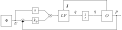
\includegraphics[width=\textwidth,height=\textheight,keepaspectratio]{ctrsyst.png}
  \captionof{figure}{Структурная схема следящей системы.}
  \label{}
\end{center}

Получив решение обратной скоростной задачи мы получили возможность синтезировать управления заданного 6-скоростью объекта положения звена. Однако, обычно, целью позиционера является управлением положением звена, а не его скоростью.

Прямое решение задачи управления положением через интеграл скоростного управления, очевидно, очень быстро приведет к накоплению вычислительной ошибки.

Чтобы исключить вычислительную ошибку зададимся модельным положением управляемого звена. Пусть задача траекторного управления вырабатывает уставку в виде текущих объектов положения $U(t)$ и скорости $\dot{U}(t)$.

Используем объект уставки как основной сигнал управления (прямое управление), а объект положения для вычисления ошибки $E(t)$ в цепи обратной связи.

Тогда система управления будет отрабатывать управляющее воздействие $\dot{U}(t)$, замешивая в него с небольшим коэффициентом ошибку по положению $E(t)$.

Компенсация $E(t)$ вносится в форме 6-вектора положения взвешенного на соответствующий коэффициент усиления.\ref{geom}. 

Если сумирование компоненты линейной скорости уставки и взвешенного сигнала ошибки положения не вызывает вопросов в силу линейности преобразований координат и линейных скоростей, то сумирование компонент угловой скорости и взвешенных компонент вектора поворота необходимо обосновать.

Возьмём вектор компенсации $\Omega_e$ сонаправленный сигналу ошибки углового положения $\rho_e$ и равный по модулю $K|\rho_e|$, где $K$ размерный коэффициент приведения.
Разложим вектор компенсации $\Omega_e$ на аксиальную и тангенсальную к вектору $\omega_u$ направления.   

Тогда сумарный вектор угловой скорости будет иметь вид 
\begin{equation}
\omega = |\omega_u + \omega_e^tang|\bar{t} + |\omega_e^norm|\bar{n}
\end{equation} 
Тангенсальная компонента $\omega_e^tang$ прямо корректирует модуль $\omega_u$, ускоряя или замедляя воздействие исходя из текущей ошибки. Компонент $\omega_e^norm$ подворачивает звено к ориентации модельного положения. В силу ортогональности управления по тангенсальному и нормальному ортам можно считать независимым при достаточно малом вычислительном шаге.

Надо отметить, что ошибка углового положения более неприятна для системы в целом, поскольку приводит к повороту базиса и переносу ошибки на компоненты линейного положения. Соответственно, следует либо устанавливать высокие требования к динамической точности такой системы, либо осуществлять предобработку сигнала управления путём переноса в связанный базис. 

Анализ устойчивости такой системы управления выходит за рамки настоящего изложения.

Следует также отметить, что может быть построена система управления исключительно по сигналу $E(t)$ без прямого управления по $U(t)$. Такая система имеет лучшую устойчивость и не имеет проблемы переноса ошибки углового положения на компоненты линейного, но имеет худшее быстродействие и может иметь статическую ошибку в режиме движения с ненулевой скоростью.

%\newpage
\section{Построение масива траекторных точек для решения задачи линейной интерполяции.}

Многие практические задачи, связанные с применением роботов манипуляторов, позиционеров и прочих подобных изделий не требуют синтеза управления в реальном времени. Вместо этого используется линейная интерполяция по заранее заданному массиву геометрических точек, между которыми манипулятор перемещается задавая постоянную скорость управления по кинематическим координатам. Этот массив или просчитывается незадолго до начала движения, либо вообще формируется один раз для всех последующих циклов работы механизма, если задача может быть описана циклом.

Несмотря на то, что целью настоящего метода не является построение интерполяционных массивов, мы можем использовать его для этой цели.

Разберём построение массива точек для прохода по траектории. Зададим положение и ориентацию управляемого звена как функцию времени $P(t)$. Прогоним математическую модель системы управления по этой траектории и с заданным дискретом (по времени или расстоянию) зафиксируем компоненты вектора $q(t_i)$, $i=0..n$. Массив векторов $q(t_i)$ есть искомый массив точек.

Компоненты массива могут содержать небольшую ошибку позиционирования, которую можно выбрать методом координатного спуска или запустив модель в режими стабилизации к соответствующему моменту $t$ траекторному положению.

Дальнейший проход по заданному таким образом массиву точек в общем случае имеет ошибку на интерполяционных участках. Для ее минимизации следует уменьшать интервал.

%\newpage
\section{Учет ограничений и весов на уровне координатного решателя. Метод исключения координат.}

При том, что концептуально учет ограничений должен производится на уровне траекторного решателя и приблизительно формулироваться как <<Вышестоящей системе не следует задавать управления, которое нижестоящая не может выполнить>>, полезно рассмотреть возможности внесения ограничений на уровне кординатного решателя.

Как было указано ранее в разделе \ref{invspd_sect}, есть множество вариантов выбора коэффициентов линейной комбинации, удовлетворяющих заданной траектории. Выбор конкретной комбинации зависит от выбранного математического метода и его параметров. Имея на входе 6-вектор потребной скорости, а на выходе вектор производных кинематических координат, координатный решатель с точки зрения остальной системы представляет собой черный ящик и слабо связан с её работой в целом.

Таким образом, изменяя внутреннее устройство координатного решателя мы можем добиться поведения системы, учитывающего необходимые ограничения.
\begin{equation}
\dot{q}(t) = F(V(t), Z(q,\dot{q},t)) 
\end{equation}, где F - функция координатного решателя, а $Z(q,\dot{q},t))$ - дополнительные аргументы, учитывающие текущие ограничения.   

Возможности введения ограничений напрямую зависит от выбраного $F$ метода метода решения поиска комбинации. Некоторые классы рассматриваемых ограничений не могут быть достигнуты при одном выборе функции $F$, но могут быть достигнуты при другом. Исходя из этого, конкретный выбор $F$ должен осуществляться из соображений оптимальности вычислительной реализации в конкретном решателе и возможности учёта необходимых ограничений.

В разделе \ref{invspd_sect} были рассмотрены два метода поиска вектора коэффициентов линейной комбинации. Рассмотрим возможность внесения ограничений в каждый из них.

Метод координатного спуска достаточно легко подвергается модификации и имеет множество параметров. Мы можем варьировать множители для спуска по конкретным координатам вплоть до возможности обнуления приращения в случае, если скалярное произведение целевого 6-вектора и 6-вектора чувствительности по соответствующей координате направлены в неудобную сторону, например если дальнейшее движение по этой координате приведет к столкновению с ограничителем. Метод координатного спуска позволяет достаточно вольно учитывать ограничения и удобен для их внесения. Анализ конкретных алгоритмов введения весов и ограничений выходит за рамки настоящего изложения. 

Метод решения СЛАУ через поиск псевдообратной матрицы гораздо более строг алгоритмически и не позволяет такого вольного обращения с собой, как метод координатного спуска. Однако и здесь мы можем рассмотреть некоторые возможности влиять на результат вычисления.

Один из возможных способов выполнить ограничения на координату
\begin{equation}
q^i_{min} < q^i < q^i_{max} 
\end{equation} является метод исключения координаты. При его использовании, если решение СЛАУ даёт $\dot{q}^i$ такое что, $q^i$ стремится покинуть рабочую зону, мы исключаем координату $q^i$ из вектора кинематических параметров и проводим решение СЛАУ повторно. $\dot{q}^i$ при этом считается равным нулю на текущей итерации. Следует учесть, что такой метод может приводить к резкому останову и не быть приемлемым.

Автор полагает, что может быть найден метод решения поиска поиска линейной комбинации, лучше подходящий для внесения весов и ограничений, вместе с тем достаточно хороший для вычислительной реализации в ЦПУ или ПЛИС.

Особый интерес представляет поиск такого алгоритма, в котором положительная и отрицательная скорости по каким-либо координатам будут иметь разные веса. 

Удобно то, что декомпозиция на траекторную и координатную задачи позволяет эксперементировать с координатным алгоритмом независимо от архитектуры системы в целом.

%\newpage
\section{Учет ограничений на уровне траекторного решателя. Разбиение кинематической цепи.}\label{restr_traj}

Очевидным ограничением траекторного управления выходным звеном кинематической цепи является недопустимость выхода положения уставки за границы досягаемости манипулятора. Построение зоны допустимых положений манипулятора как правило является достаточно простой задачей и зачастую для ее решения достаточно проанализировать движение в условиях крайних положений нескольких обобщенных координат.

Более сложным вопросом является недопущение самопересечений (внутренних столкновений) звеньев цепи, но на практике такая проблема возникает не часто, в силу того, что сильно кинематически избыточные системы не применяются на практике.

Если же в силу избыточности кинематической цепи координатный алгоритм приводит кинематическую цепь в неслишком естественное положение, положение характеризуемое большой нагрузкой или, возможно сингулярным состоянием, мы можем озаботится дополнительными параметрами управления, тем самым снижая свободу цепи. Радикальным методом решения этой проблемы будет исключения части координат из вектора синтезируемого управления на специальных режимах работы, или использование разных участков кинематической цепи для решения разных задач. 

Рассмотрим другой вариант решения этой задачи


%\newpage
\section{Управление манипулятором в движущемся локальном базисе.}

На основе субъективных ощущений можно сделать вывод, что человек и, интерполируя, прочие живые организмы, имеющие организацию двигательных подсистем мозга близких к нам строят геометрические модели окружающего мира на основе органов чувств с центрами в районе головы (сенсорная модель), и туловища (двигательная модель).

Эти геометрические модели используются для управления конечностями в условиях

%\newpage 
\section{Совместное управление частично пересекающимися кинематическими цепями. Древовидная кинематическая цепь.}

Древовидная кинематическая цепь является сложной кинематической цепью. Ее матрица частных производных скоростей $J$ может быть построена на основе анализа простых подцепей, входящих в нее. Древовидная цепь (как и было указано в разделе \ref{other}) не имеет верхнетреугольного вида, как простая, но в целом процесс построения матрицы $J$ для нее не сильно отличается.

Ярким примером задачи управления древовидной кинематической цепи является задача совместного управления положением пальцев руки. Хотя автор и не возьмётся утверждать, что живые организмы комплексно решают задачу управления пальцами конечностей, можно показать, что такое управление возможно и реализуемо в рамках настоящего метода.

Задача управления древовидной цепью может быть решена через разбиение сложной цепи на несколько иерархически связанных простых подцепей, управление по которым может осуществляться независимо, но совместное управление позволяет добиться лучшего качества регулирования.

Для построения такого решения построим матрицу $J$ и выберем в качестве управляемых компонент компоненты скоростей выходных звеньев древовидной кинематической цепи. Следует оговориться, что для задачи управления кистью в достаточной степени бессмысленно пытаться управлять ориентацией каждого пальца. Вместо этого можно взять в качестве управляемых компонент линейные компоненты скоростей кончиков захватов и угловую ориентацию кисти. 

Теперь, в соответствии с методикой изложенной в \ref{inverse_sect} мы можем построить решение обратной скоростной задачи.

%\newpage

\section{Выводы.}
Дальнейшее развитие робототехнических систем, в частности антропоморфных роботов, роботов обладающих сложным поведением требует внедрения методов управления движения претендующих на определённую общность, допускающих возможность решения широкого круга задач при учете широкого и, возможно, заранее неизвестного класса ограничений на управляющее воздействие.

Декомпозиция задачи позволяет.

\end{document}

